\documentclass[tikz,border=4pt]{standalone}
% Shared visual grammar: role fills, dark connectors, and 7-point typography.
% Build each standalone figure from this directory. No external images required.
\pdfinfoomitdate=1
\pdftrailerid{}
\usepackage[T1]{fontenc}
\usepackage{helvet}
\renewcommand{\familydefault}{\sfdefault}
\usepackage{amsmath,amssymb}
\hyphenpenalty=10000
\exhyphenpenalty=10000
\usetikzlibrary{arrows.meta,calc,fit,positioning,decorations.pathreplacing,backgrounds}
\definecolor{ink}{HTML}{172B3A}
\definecolor{muted}{HTML}{586D85}
\definecolor{datafill}{HTML}{F1F5F9}
\definecolor{dataline}{HTML}{62748E}
\definecolor{modelfill}{HTML}{E5E9FF}
\definecolor{modelline}{HTML}{7887C7}
\definecolor{llmfill}{HTML}{FFE4E8}
\definecolor{llmline}{HTML}{E68494}
\definecolor{truthfill}{HTML}{D0FAE5}
\definecolor{truthline}{HTML}{35A782}
\newcommand{\seven}{\fontsize{7}{8.5}\selectfont}
\tikzset{
 every node/.append style={font=\seven,text=ink,align=center},
 box/.style={draw=dataline,fill=white,rounded corners=3pt,line width=.65pt,inner sep=5pt,minimum height=8mm},
 data/.style={box,fill=datafill},
 model/.style={box,draw=modelline,fill=modelfill},
 llm/.style={box,draw=llmline,fill=llmfill},
 truth/.style={box,draw=truthline,fill=truthfill},
 title/.style={font=\seven\bfseries,inner sep=1pt},
 word/.style={text=muted,inner sep=1pt,align=center},
 label/.style={fill=white,inner xsep=2pt,inner ysep=1pt,text=muted},
 flow/.style={-{Stealth[length=2.4mm,width=1.9mm]},draw=ink,line width=1.2pt,shorten >=1.5pt},
 branch/.style={-{Stealth[length=2mm,width=1.6mm]},draw=ink,line width=.9pt,shorten >=1pt},
 route/.style={draw=ink,line width=1.2pt},
 update/.style={-{Stealth[length=2.2mm,width=1.7mm]},draw=modelline,line width=1pt,dash pattern=on 3pt off 2pt,shorten >=1.5pt},
 boundary/.style={draw=dataline,dash pattern=on 3pt off 2pt,rounded corners=3pt,line width=.6pt},
 chip/.style={minimum height=4mm,inner xsep=3pt,inner ysep=1.5pt,rounded corners=2pt},
}
% Optional role key. Anchor at the center of an uncluttered final row.
\newcommand{\rolekey}[2]{
 \node[word,anchor=east] at (#1-6.6,#2) {\textit{Key}};
 \node[data,chip] at (#1-5.2,#2) {records / data};
 \node[model,chip] at (#1-1.9,#2) {learned model / policy};
 \node[llm,chip] at (#1+1.65,#2) {LLM signal};
 \node[truth,chip] at (#1+4.95,#2) {labels / evaluation};
}

\begin{document}
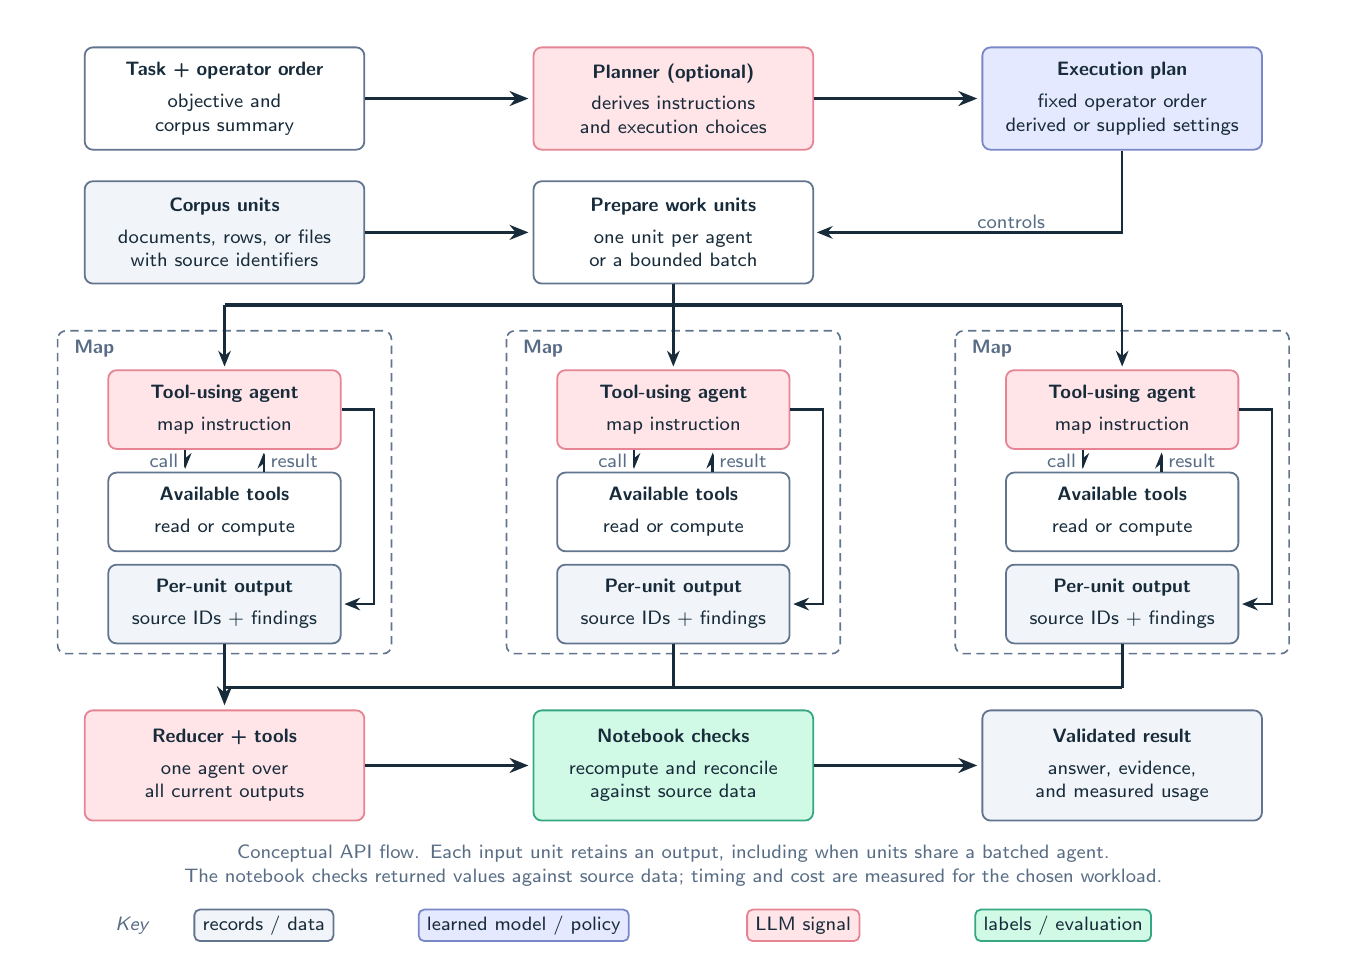
\begin{tikzpicture}

\useasboundingbox (-.2,.3) rectangle (16.2,-11.35);
\node[box,text width=32mm,minimum height=13mm] (task) at (2.3,-.6) {\textbf{Task + operator order}\\[3pt]objective and\\corpus summary};
\node[llm,text width=32mm,minimum height=13mm] (planner) at (8,-.6) {\textbf{Planner (optional)}\\[3pt]derives instructions\\and execution choices};
\node[model,text width=32mm,minimum height=13mm] (plan) at (13.7,-.6) {\textbf{Execution plan}\\[3pt]fixed operator order\\derived or supplied settings};
\draw[flow] (task) -- (planner);
\draw[flow] (planner) -- (plan);

\node[data,text width=32mm,minimum height=13mm] (corpus) at (2.3,-2.3) {\textbf{Corpus units}\\[3pt]documents, rows, or files\\with source identifiers};
\node[box,text width=32mm,minimum height=13mm] (work) at (8,-2.3) {\textbf{Prepare work units}\\[3pt]one unit per agent\\or a bounded batch};
\draw[flow] (corpus) -- (work);
\draw[branch] (plan.south) |- node[label,pos=.68,above] {controls} (work.east);

\draw[route] (work.south) -- (8,-3.22);
\draw[route] (2.3,-3.22) -- (13.7,-3.22);

\foreach \x/\i in {2.3/1,8/2,13.7/3} {
  \draw[boundary] (\x-2.12,-3.55) rectangle (\x+2.12,-7.65);
  \node[word,anchor=west] at (\x-1.95,-3.78) {\textbf{Map}};
  \node[llm,text width=26mm,minimum height=10mm] (agent\i) at (\x,-4.55) {\textbf{Tool-using agent}\\[3pt]map instruction};
  \node[box,text width=26mm,minimum height=10mm] (tool\i) at (\x,-5.85) {\textbf{Available tools}\\[3pt]read or compute};
  \node[data,text width=26mm,minimum height=10mm] (finding\i) at (\x,-7.02) {\textbf{Per-unit output}\\[3pt]source IDs + findings};
  \draw[branch] (\x,-3.22) -- (agent\i.north);
  \draw[branch] ([xshift=-5mm]agent\i.south) -- node[label,left] {call} ([xshift=-5mm]tool\i.north);
  \draw[branch] ([xshift=5mm]tool\i.north) -- node[label,right] {result} ([xshift=5mm]agent\i.south);
  \draw[branch] (agent\i.east) -- (\x+1.9,-4.55) -- (\x+1.9,-7.02) -- (finding\i.east);
  \draw[route] (finding\i.south) -- (\x,-8.08);
}

\draw[route] (2.3,-8.08) -- (13.7,-8.08);
\node[llm,text width=32mm,minimum height=14mm] (reduce) at (2.3,-9.07) {\textbf{Reducer + tools}\\[3pt]one agent over\\all current outputs};
\node[truth,text width=32mm,minimum height=14mm] (check) at (8,-9.07) {\textbf{Notebook checks}\\[3pt]recompute and reconcile\\against source data};
\node[data,text width=32mm,minimum height=14mm] (answer) at (13.7,-9.07) {\textbf{Validated result}\\[3pt]answer, evidence,\\and measured usage};
\draw[flow] (2.3,-8.08) -- (reduce.north);
\draw[flow] (reduce) -- (check);
\draw[flow] (check) -- (answer);

\node[word,text width=145mm] at (8,-10.34) {Conceptual API flow. Each input unit retains an output, including when units share a batched agent.\\The notebook checks returned values against source data; timing and cost are measured for the chosen workload.};
\rolekey{8}{-11.1}

\end{tikzpicture}
\end{document}
